%--------------------------------------------------------------------------------
%\documentclass{article}

\documentclass[12pt]{article}
\usepackage[T1]{fontenc} 
\usepackage[bf]{caption}
\usepackage{hyperref}
\usepackage[all]{hypcap}
\usepackage[utf8]{inputenc}
\usepackage{graphicx}
\usepackage[czech, english]{babel}
\selectlanguage{english}
\usepackage{subfig}                % \subfloat
\usepackage{color}
\usepackage{subfigure}
\usepackage{url}
\inputencoding{utf8}
%\usepackage[bf]{caption2}
\usepackage{hyperref}
\usepackage[all]{hypcap}
\hypersetup{colorlinks=false, linkbordercolor=1 1 1, citebordercolor=1 1 1}
\usepackage[right]{lineno}
\renewcommand\linenumberfont{\normalfont\tiny\color{blue}}
\usepackage[style=numeric]{biblatex}
\addbibresource{project.bib}
\usepackage[a4paper, margin=1in]{geometry}
\usepackage{amsmath}
\usepackage{float}



\title{Road segmentation from satellite images}
\author{Ondrej Kováč (xkovac57) \and Jakub Július Šmýkal (xsmyka01) \and Jan Svoboda (xsvobo2b)}
\date{\today}


%--------------------------------------------------------------------------------


\begin{document}
\selectlanguage{english}
\maketitle

\section{Introduction}
This work focuses on road segmentation from satellite images. It contains the process of implementation, training and testing of various convolutional neural networks, which are able to identify and create masks for roads in satellite images. Road segmentation can be useful in many areas, such as urban planning, disaster response, autonomous navigation and so on.

%%%%%%%%%%%%%%%%%%%%%%%%%%%%%%%%%%%%%%%%%%%%%%%%%%%%%%%%%%%%%%%%%%%%%%%%%%%%%%%%%%%%%%%%

\section{Existing solutions}
As this is an image segmentation task, it was obvious to us, that we would be using a convolutional neural network. We looked at 3 different papers \cite{ref1}\cite{ref2}\cite{ref3} focusing on this specific issue and found, that they use very similar approaches. Namely, all of them used some variation of the U-Net architecture. 

\begin{figure}[h]
  \centering
  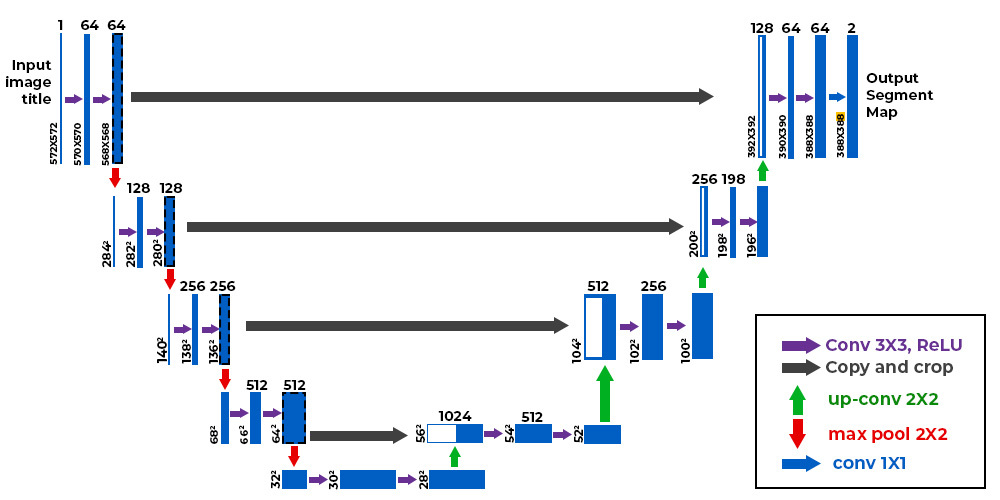
\includegraphics[scale = 0.35]{unet.png}
  \caption{U-Net architecture example. Sourced from \cite{g4g}}
  \label{fig:obrazek}
\end{figure}

U-Net is an architecture specifically designed for image segmentation tasks and consists of two main parts:

\begin{itemize}
    \item Encoder - captures context and features from the input image through a series of convolutional and pooling layers, reducing the spatial dimensions while increasing feature depth.
    \item Decoder - Restores spatial resolution through up-convolutions (transposed convolutions) and combines these with high-resolution features from the encoder using skip connections, which help preserve spatial details.
\end{itemize}

The papers used different combinations of loss functions (Dice Loss, BCE...) and optimizers. All of them, however, had one evaluation metric in common, and that was Intersection over Union (IoU).

\[
\text{IoU} = \frac{|\text{Prediction} \cap \text{Ground Truth}|}{|\text{Prediction} \cup \text{Ground Truth}|}
\]

If we compare their results using the mean IoU metric over the testing dataset we get the following results:

\begin{itemize}
    \item Paper \cite{ref1} tested 5 different U-Net architectures:
    \begin{itemize}
        \item U-Net - 0.599
        \item ResUNet - 0.600
        \item AttUNet - 0.616
        \item C-UNet - 0.635
        \item Their Proposed U-Net model - 0.620
    \end{itemize}
    \item Paper \cite{ref2} reached an IoU of 0.73
    \item Paper \cite{ref3} tested a U-Net with 4 different backbones:
    \begin{itemize}
        \item ResNet18 - 0.711
        \item ResNet34 - 0.717
        \item ResNet50 - 0.735
        \item ResNet152 - 0.732
    \end{itemize}
\end{itemize}

These values, of course, cannot be compared directly, as the models were not trained and tested on the same data. The results do however give us an idea about the difficulty of this task. These scores, if taken at face value, actually seem quite low. We will get into the hypothesized reasons why IoU scores in this particular problem are relatively low when we explain our own model.

\section{Our Implementation}

\subsection{Goal}
As the goal of our project, we decided to test multiple different architectures and learning methods and compare their performance. Then we selected the best-performing combination and properly trained it to see if it could compare with existing solutions mentioned in the previous chapter.

\subsection{Environment}
We decided to create our project\footnote{\href{https://github.com/JuliusJx/POVa-Road-Segmentation}{GitHub Repository}} in Python and use the \textbf{Pytorch} library for our neural network. We then tested models from \textbf{Python Segmentation Models} library \cite{segmodels}. 

\subsection{Dataset}
We decided to use the \textbf{DeepGlobe Road Extraction Dataset} \cite{dataset}. This dataset contains more than 6000 training images with corresponding ground truth masks.

\subsection{Data augmentation}
We used online augmentations during training. Each time an image from the training set was augmented using the \textbf{Albumentations} library. This meant that the model was trained and evaluated on a slightly different dataset each epoch.

These augmentations modify the resolution and the color of images. Random part with user-selected resolution is cut out of the original image and randomly rotated. This newly created image has then modified color tone. There are also some additional augmentations, which are optional and can be used to create even more diverse training data. These are addition of blur, randomly adjusting brightness, contrast, saturation and hue and transformation of the image to grayscale.  

\begin{figure}[h]
    \centering
    \subfigure{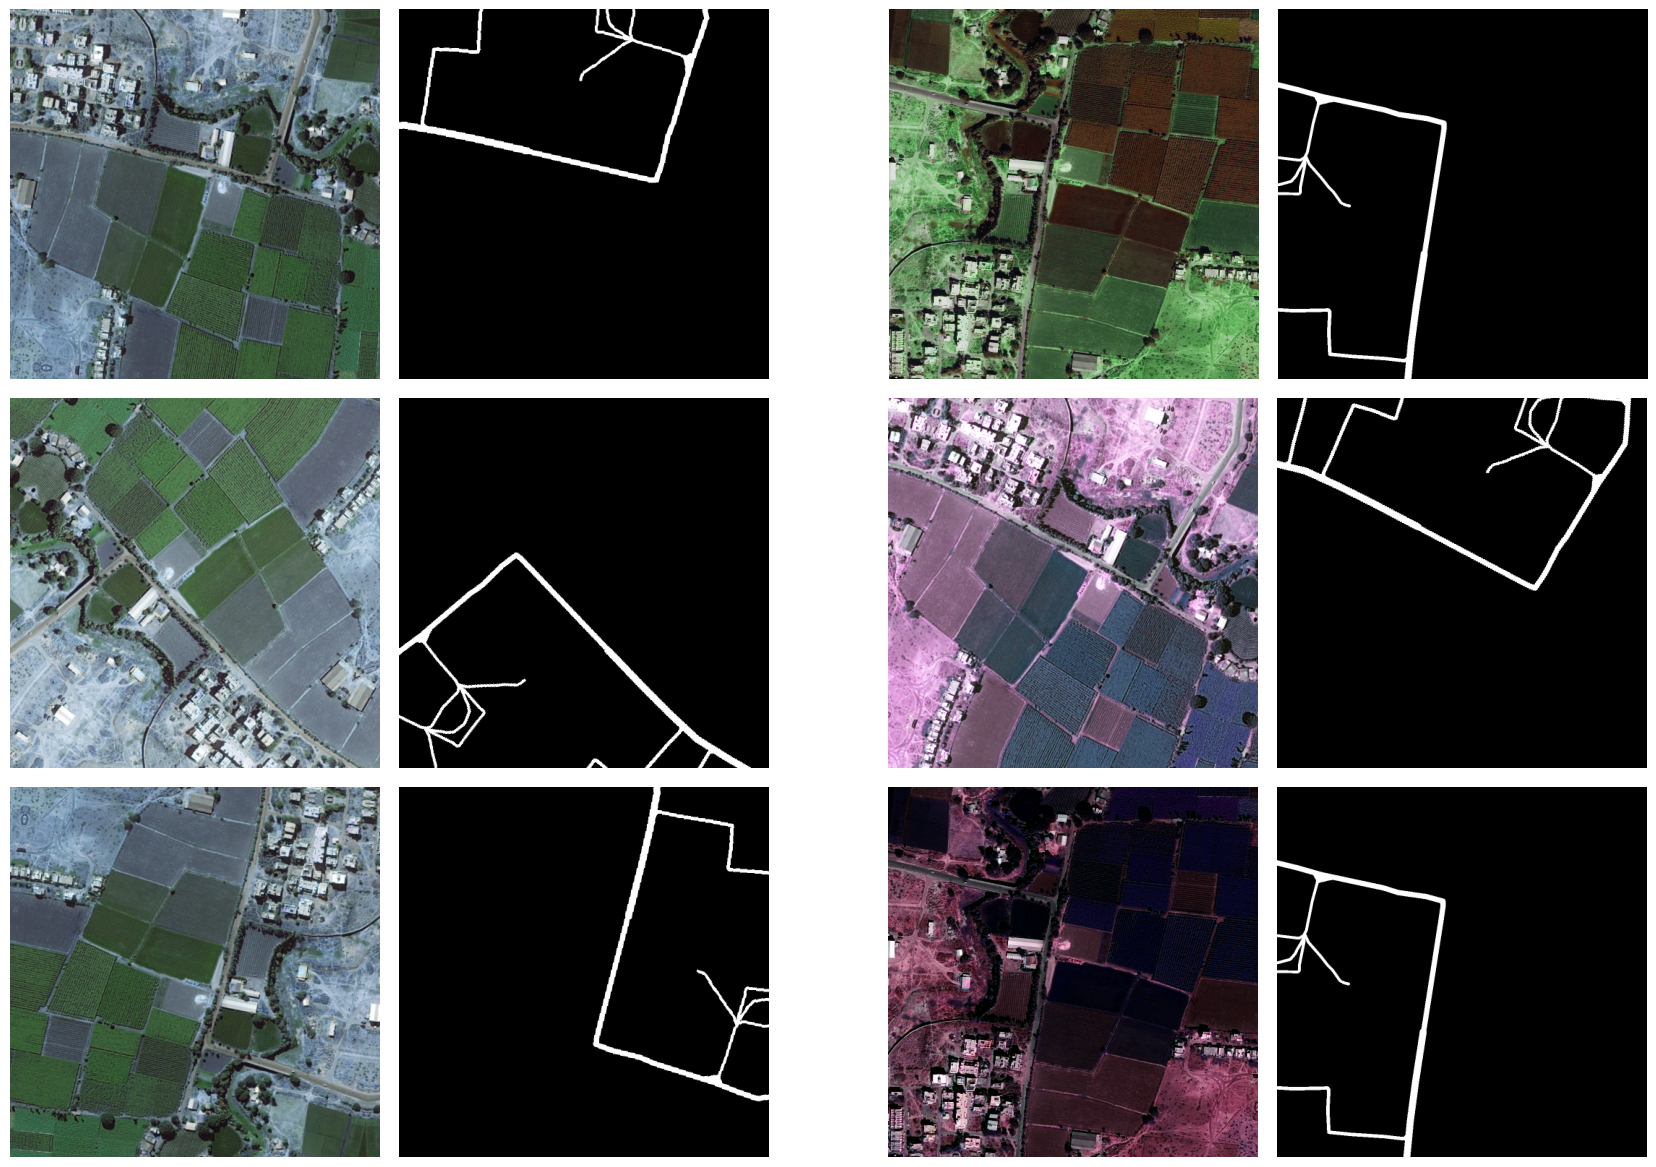
\includegraphics[width=0.7\textwidth]{doc_augmentations.png}} 
    \caption{Examples of image and its mask after multiple augmentations. Images on the right side are created with more extensive augmentations enabled.}
    \label{augmentations}
\end{figure}





%%%%%%%%%%%%%%%%%%%%%%%%%%%%%%%%%%%%%%%%%%%%%%%%%%%%%%%%%%%%%%%%%%%%%%%%%%%%%%%%%%%%%%%%

\section{Training and testing}

For the training, we used Dice's loss function. For the accuracy evaluation, we used the intersection of unions metrics (IoU). We found out that IoU was sometimes low in comparison to the quality of the graphical results. When comparing the images, we observed that the quality of the dataset was not very good, as the visually present paths were often not labeled in the dataset, as can be seen in figure \ref{missing_path}. This also caused problems in the training because the model was penalized for correctly segmented paths. Another problem is that paths can be very thin, so even a small deviation can cause a large drop in the IoU.


\begin{figure}[H]
    \centering
    \subfigure{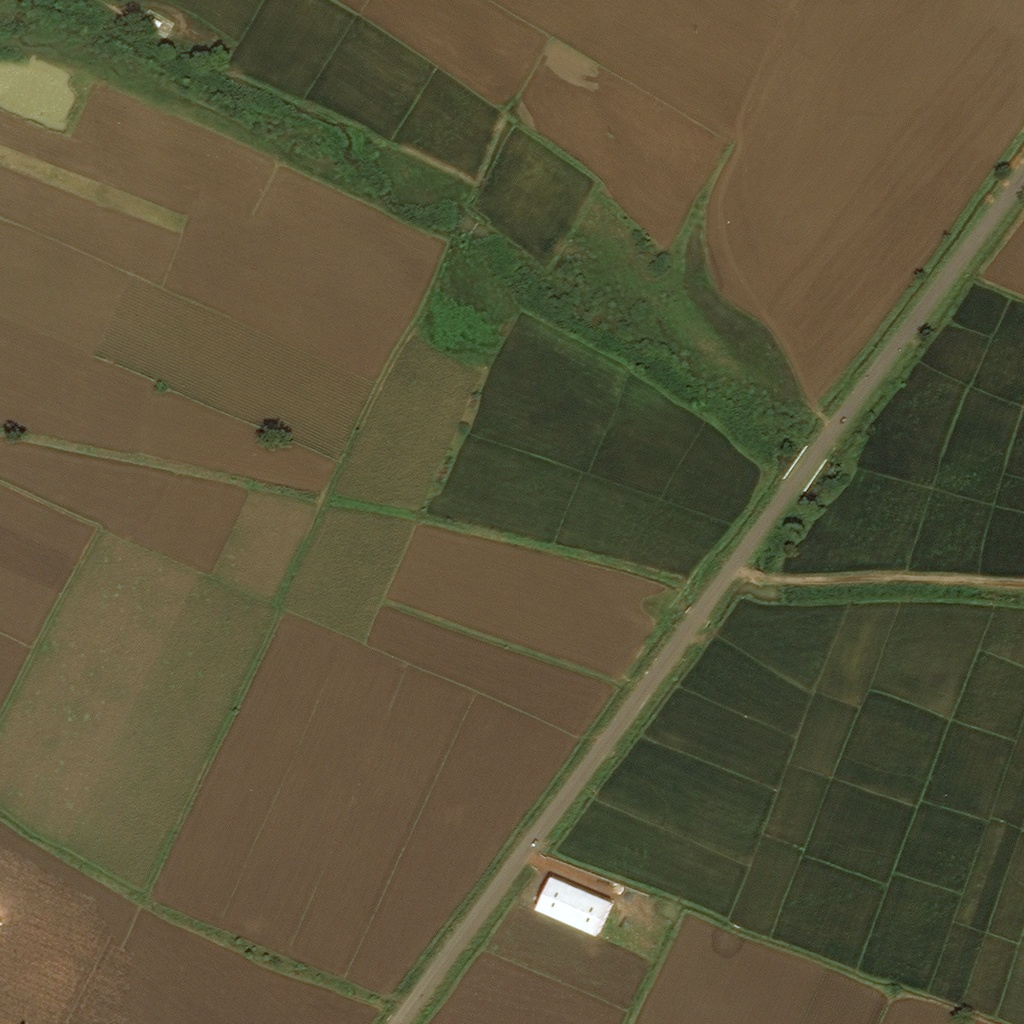
\includegraphics[width=0.3\textwidth]{499198_sat.jpg}} 
    \subfigure{
\includegraphics[width=0.3\textwidth]{499198_mask.png}} 
    \caption{Missing path example.}
    \label{missing_path}
\end{figure}


\subsection{Encoder testing}
The encoders resnet101, efficientnet-b4, and efficientnet-b5 were tested on 720 training and 180 validation images. We used pretrained weights. Training was performed on the UNET architecture in 100 epochs and for each epoch, 3 random augmentations of size 256x256 were created from each image and used for training. Finally, 100 images were tested in full size (scaled but without cropping). A comparison of the different encoders is shown in the table \ref{table_encoder_tests}.

\begin{table}[H]
    \centering
    \begin{tabular}{|l|c|c|c|}
        \hline
         Encoder & Training Loss & Training IoU & Testing IoU \\ \hline
         resnet101 & 0.360 & 0.486 & 0.457 \\
         efficientnet-b4 & 0.258  & 0.606 & 0.541  \\
         efficientnet-b5 & 0.258 & 0.607 & 0.554 \\
         \hline
    \end{tabular}
    \caption{Encoder testing results.}
    \label{table_encoder_tests}
\end{table}

It turned out that eficientenet-b5 performed the best.
When comparing the graphical outputs, eficientnet-b5 showed very good results so no other encoders were tested and this encoder was used in further experiments. Graphical results of this test can be seen in figure \ref{figure_encoder_tests}. 

\begin{figure}[h]
    \centering
    \subfigure{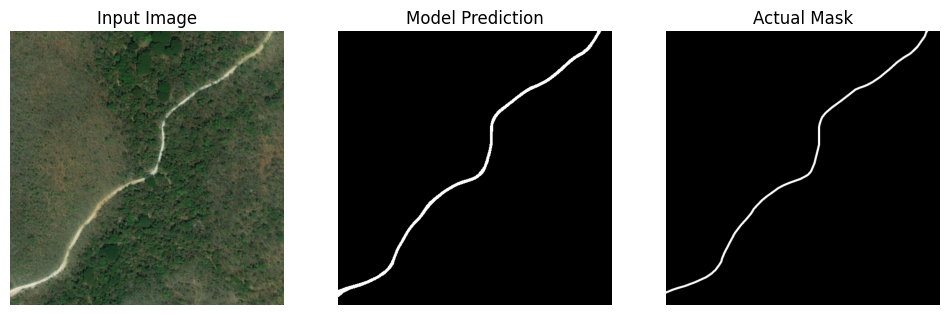
\includegraphics[width=0.65\textwidth]{cesta_efb5_fast.png}} 
    \subfigure{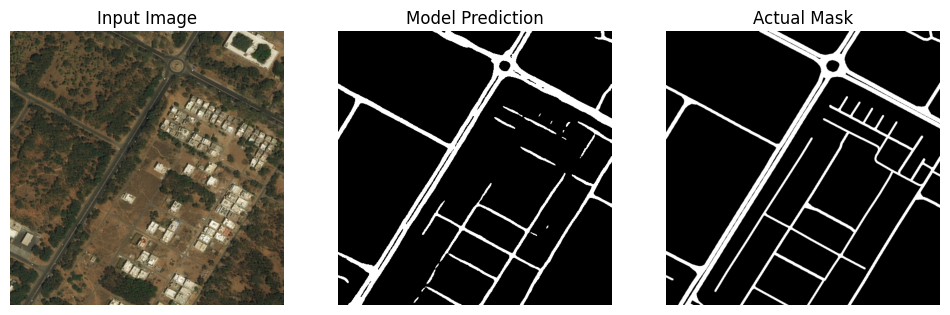
\includegraphics[width=0.65\textwidth]{kruhac_efb5_fast.png}} 
    \subfigure{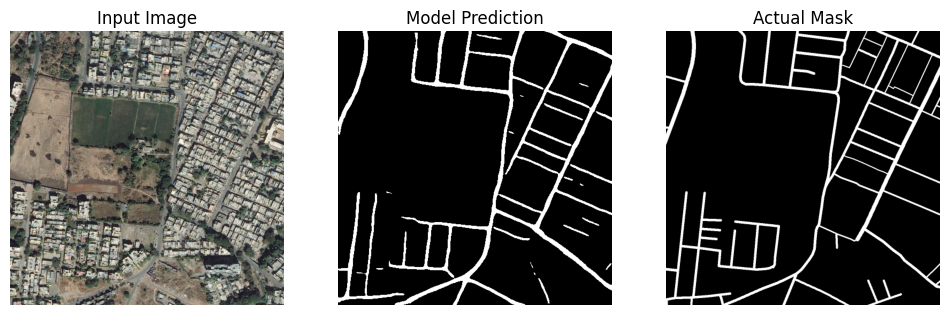
\includegraphics[width=0.65\textwidth]{mesto_efb5_fast.png}}
    \subfigure{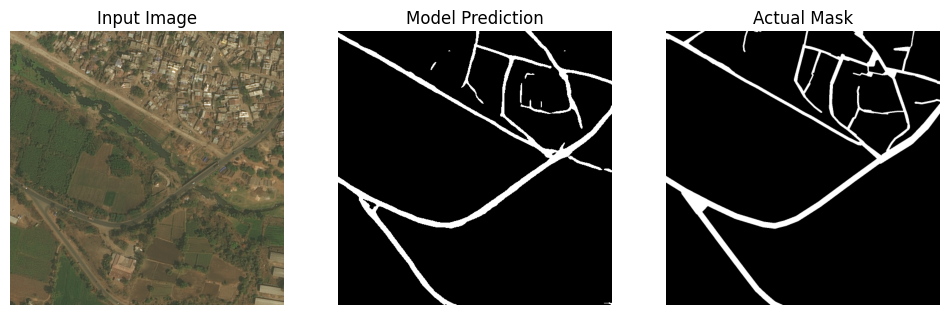
\includegraphics[width=0.65\textwidth]{mesto2_efb5_fast.png}}
    \caption{Encoder testing efficientnet-b5 results.}
    \label{figure_encoder_tests}
\end{figure}

\subsection{Architecture testing}

For testing, we decided to test all architectures available from the Python Segmentation Models library except LinkNet in the same way as the encoders. The results can be seen in the table \ref{table_encoder_tests}.


\begin{table}[H]
    \centering
    \begin{tabular}{|l|c|c|c|}
        \hline
         Model & Training Loss & Training IoU & Testing IoU \\ \hline
         FPN & 0.249 & 0.621 & 0.529  \\
         PSPNet & 0.309  & 0.554 & 0.431  \\
         PAN & 0.259 & 0.613 & 0.507 \\
         UNET & 0.258 & 0.607 & 0.554 \\
         \hline
    \end{tabular}
    \caption{Architecture testing results.}
    \label{table_encoder_tests}
\end{table}

In the table, it can be seen that FPN has the best training parameters, but it has worse results on the testing images. The visual result was also blurrier and less detailed. In the test images, UNET achieved the best results, but the PAN model converged faster in the first few epochs. The visual results were also promising for PAN after a few epochs. In the final results, the PAN has worse results than UNET. It can be caused by different resistance to errors in the training dataset. It's also good to mention that PAN is much slower than UNET.

\subsection{Final testing}

For the final testing, we used the UNET architecture with the efficientnet-b5 encoder. We used 2480 images for training, 620 for validation and we trained the model for 150 epochs. The training curve can be seen on figure \ref{fig_final_loss}. Only one augmentation for each image per epoch was used. The results can be seen in the table \ref{table_final_results}.


\begin{table}[h]
    \centering
    \begin{tabular}{|l|c|}
        \hline
         Model & UNET \\ \hline
         Encoder & efficientnet-b5 \\ \hline
         Training Loss & 0.2705 \\ \hline
         Training IoU & 0.5905 \\ \hline
         Testing IoU & 0.6463\\
         \hline
    \end{tabular}
    \caption{Final model parameters.}
    \label{table_final_results}
\end{table}


\begin{figure}[h]
    \centering
    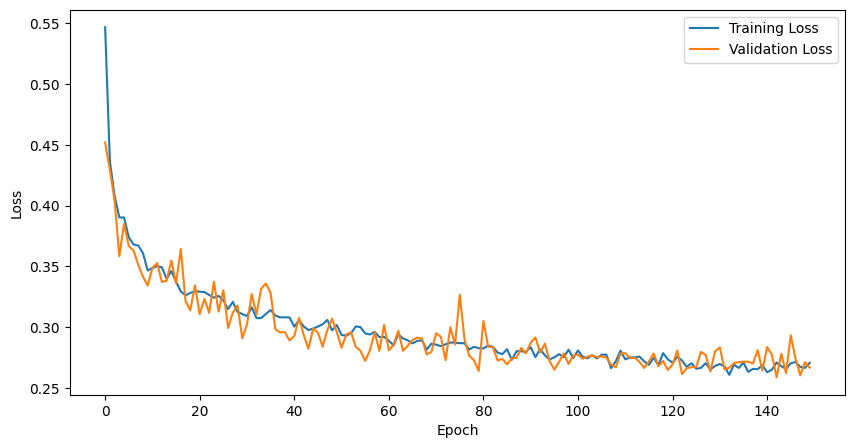
\includegraphics[width=1\linewidth]{final test training curve.png}
    \caption{Training curve for the final training.}
    \label{fig_final_loss}
\end{figure}

The graphical results can be seen in \ref{figure_final_tests}. According to the graphical results, the model performs well in path recognition and successfully ignores other structures that might resemble paths. However, in the images, it can also be seen that for thin paths, the model has trouble recognizing what is a path and what is not. We believe this is primarily due to the problematic dataset, where some paths, especially the less frequent ones, are not labeled in the dataset at all. 


\begin{figure}[h]
    \centering
    \subfigure{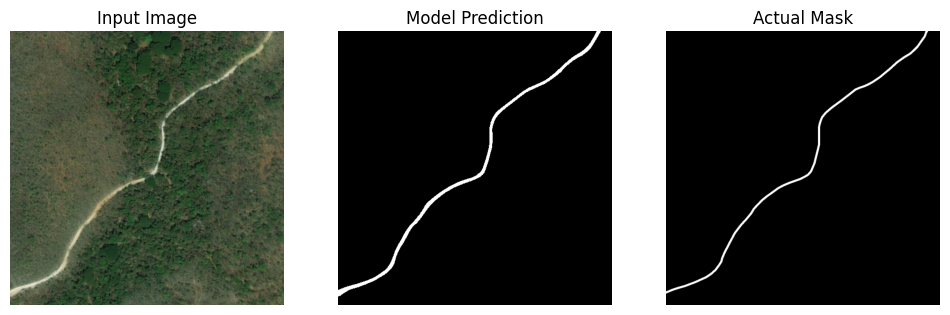
\includegraphics[width=0.7\textwidth]{cesta_finalpng.png}} 
    \subfigure{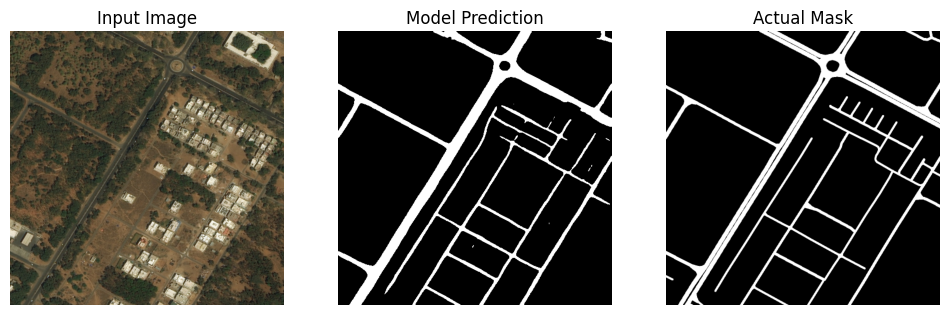
\includegraphics[width=0.7\textwidth]{kruhac_final.png}} 
    \subfigure{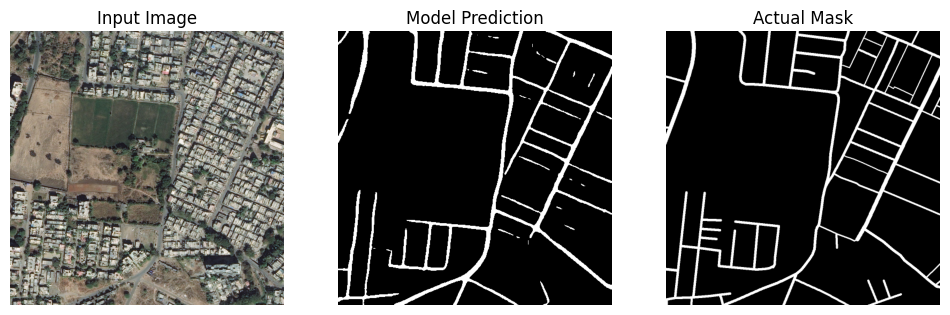
\includegraphics[width=0.7\textwidth]{mesto_final.png}}
    \subfigure{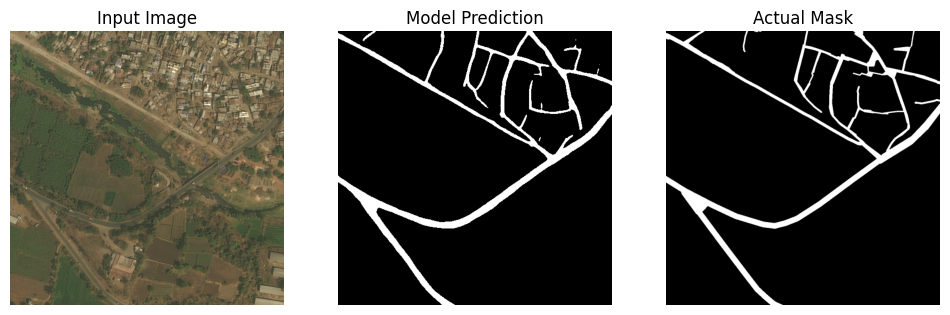
\includegraphics[width=0.7\textwidth]{mesto2_final.png}}
    \subfigure{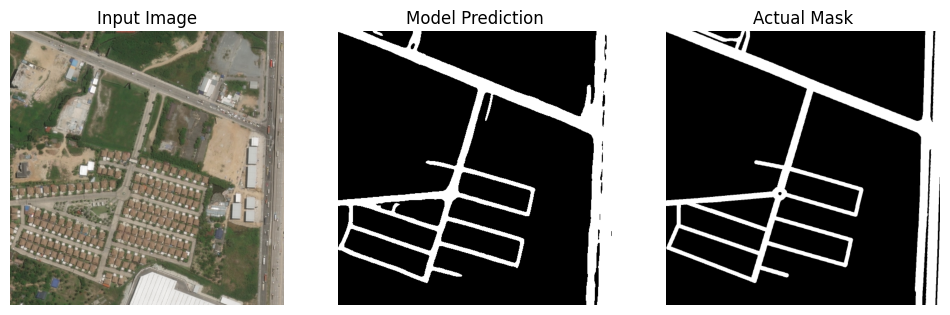
\includegraphics[width=0.7\textwidth]{mesto3_final.png}}
    \caption{Final testing results.}
    \label{figure_final_tests}
\end{figure}

\clearpage

%%%%%%%%%%%%%%%%%%%%%%%%%%%%%%%%%%%%%%%%%%%%%%%%%%%%%%%%%%%%%%%%%%%%%%%%%%%%%%%%%%%%%%%%

\section{Conclusion}
We have successfully trained a convolutional neural network for road segmentation that is able to create masks for roads in satellite images with accuracy comparable to existing models. Despite the relatively low quantitative accuracy, which can mostly be attributed to the low quality of the dataset, we are pleased with the qualitative results. Future improvements could include refining the dataset and removing samples with poor ground truth masks, which would undoubtedly make the model more accurate.


\printbibliography

%\appendix
%\newpage
%\section{}

\end{document}

